\documentclass[10pt]{beamer}

\usepackage[american]{babel}
\usepackage[utf8]{inputenc}
%\usepackage{soul}
\usepackage{amsmath}
\usepackage{amssymb}
\usepackage{textcomp}
\usepackage{listings}
\lstset{
  language=haskell,
  upquote=true,
  basicstyle=\ttfamily,          % print whole listing in typewriter
  keywordstyle=\color{blue}\bfseries, % bold blue keywords
  %identifierstyle=,           % nothing happens
  commentstyle=\color{green}, % green comments
  stringstyle=\color{red},      % typewriter type for strings
  showstringspaces=false     % no special string spaces
}
%\usepackage[all]{xy}
\usepackage{tikz}
%\usetikzlibrary{arrows,shapes,automata}
\usepackage{graphicx}
%\usepackage[bibstyle=beamer,citestyle=authoryear-comp,doi=false,isbn=false,eprint=false,maxnames=10]{biblatex}
%\bibliography{../defeo}
\usepackage{../mysymbols}
\usepackage{array}

% \usepackage[T1]{fontenc}
% \renewcommand{\rmdefault}{pplx}
% \renewcommand{\sfdefault}{uop}
% \usepackage[T1]{eulervm}

\renewcommand{\emph}[1]{{\usebeamercolor[fg]{structure}#1}}

\mode<presentation>{%
  \usetheme[]{Boadilla}
%  \usefonttheme{professionalfonts}
  \usefonttheme[onlymath]{serif}
  \usecolortheme[rgb={0.56,0.3,0}]{structure}
  \setbeamercolor{alerted text}{fg=blue}
  \setbeamertemplate{navigation symbols}{}
}


\title{Fast Algorithms for Towers of Finite Fields and Isogenies}
\author{Luca~De~Feo}
\institute[LIX \& INRIA Saclay]{LIX, École Polytechnique \& INRIA Saclay, Projet TANC}
\date[December 13, 2010]{December 13, 2010\\École Polytechnique, Palaiseau}


\AtBeginSection[]
{
  \begin{frame}<beamer>
    \frametitle{Plan}
    \tableofcontents[currentsection]
  \end{frame}
}

\begin{document}

\begin{frame}
  \titlepage
%   
\includegraphics[height=2em]{../logos/x-color.pdf}
%   \hfill
%   
\includegraphics[height=2em]{../logos/lix-color.pdf}
%   \hfill
%   
\includegraphics[height=2em]{../logos/inria-color.pdf}
\end{frame}

%%
%%

\begin{frame}
  \frametitle{The Discrete Logarithm Problem}
  
  \begin{columns}
    \begin{column}{0.4\textwidth}
      \begin{tikzpicture}
        \begin{scope}
          \foreach \alpha in {0,...,4} {
            \filldraw (-65-25*\alpha:2) circle (2pt);
          }
          \foreach \alpha in {0,...,3} {
            \draw[->] (-65-25*\alpha:2) arc (-65-25*\alpha:-85-25*\alpha:2);
            \draw (-90-25*\alpha:2.3) node {$g^\alpha$};
          }
          \draw (-65:2.3) node {$g^{n-1}$};
          \draw[densely dotted,gray] (-65:2) arc (-65:195:2);
          \draw (0,0) node {\Large $G=\langle g\rangle$};
        \end{scope}
        
        \begin{uncoverenv}<2->
          \begin{scope}[yshift=-3cm]
            \foreach \alpha in {0,...,4} {
              \filldraw (-65-25*\alpha:2) circle (2pt);
            }
            \foreach \alpha in {0,...,3} {
              \draw[->] (-65-25*\alpha:2) arc (-65-25*\alpha:-85-25*\alpha:2);
              \draw (-90-25*\alpha:2.3) node {$\alpha$};
            }
            \draw (-65:2.3) node {$n-1$};
            \draw[densely dotted,gray] (-65:2) arc (-65:48:2);
            \draw[densely dotted,gray] (132:2) arc (132:195:2);
            \draw (0,-0.5) node {\Large $\Z/n\Z$};
          \end{scope}
        \end{uncoverenv}
        
        \begin{uncoverenv}<3->
          \foreach \alpha in {0,...,4}
          \usebeamercolor[fg]{alerted text}
          \draw[dashed] (-65-25*\alpha:2) -- ++(0,-3cm);
        \end{uncoverenv}
      \end{tikzpicture}
    \end{column}
    \begin{column}{0.6\textwidth}
      \begin{block}{Exponentiation in a cyclic group}
        Let $G=\langle g\rangle$ be a cyclic group of order $n$.
        Define
        \begin{align*}
          \exp_g : \Z/n\Z &\ra G\text{,}\\
          x&\mapsto g^x\text{.}
        \end{align*}
      \end{block}

      \begin{block}<2->{Discrete logarithm} $\exp_g$ is an
        isomorphism. Its inverse is called \emph{discrete logarithm}.
        \begin{align*}
          \log_g : G &\ra \Z/n\Z\text{,}\\
          g^x&\mapsto x\text{.}
        \end{align*}

        \begin{uncoverenv}<3-> Computing it is called the
          \alert{Discrete Logarithm Problem} (DLP) of $G$.
        \end{uncoverenv}
      \end{block}
    \end{column}
  \end{columns}
\end{frame}

%%

\begin{frame}
  \frametitle{Elliptic curve cryptography}

  \begin{columns}
    \begin{column}{0.45\textwidth}
      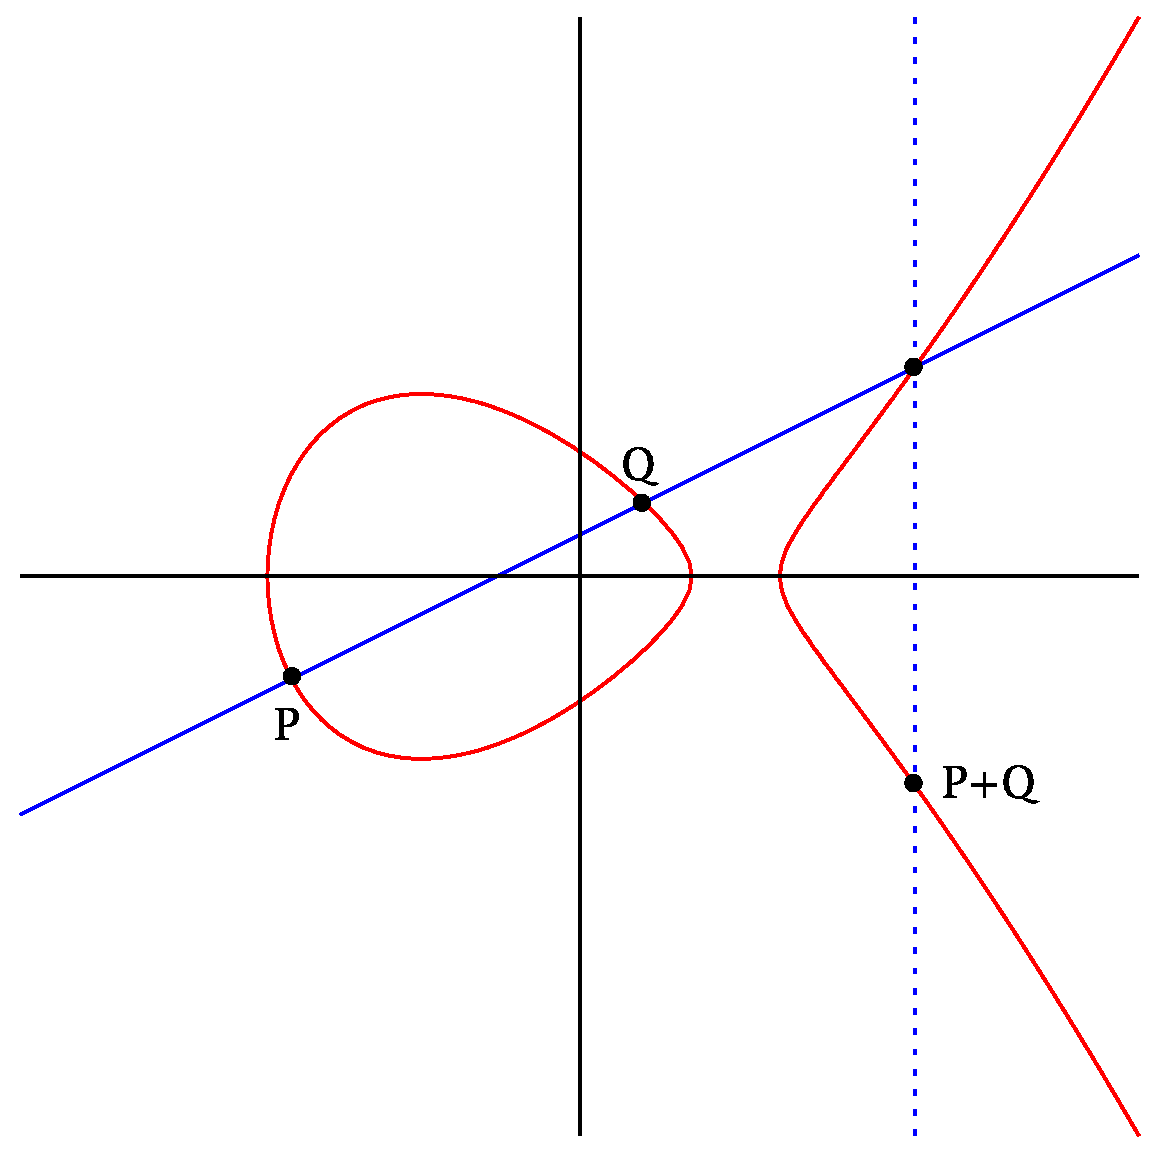
\includegraphics[width=\textwidth]{../isogeny/ec-add.pdf}
    \end{column}
    \begin{column}{0.5\textwidth}
      \begin{block}{Elliptic curve (Weierstrass form)}
        \[E : y^2 = x^3 + ax + b\text{;}\]
      
        The set of points of an elliptic curve is endowed with a group
        law via the chord-and-tangent law.
      \end{block}
    
      \begin{block}{}
        \emph{Hasse bound:} $\card{E(\F_q)} \sim q$.
      \end{block}
    \end{column}
  \end{columns}

  \begin{center}
    \begin{tabular}{l | l | l}
      &\emph{\textbf{Finite field crypto}} & \emph{\textbf{Elliptic curve crypto}}\\
      \hline
      \emph{Group} & $\F_q^\ast$ & $E(\F_q)$\\
      \emph{Protocols} & El Gamal, DSA, \dots & ECDH, ECDSA, ECMQV, \dots\\
      \emph{Key sizes}\footfullcite[Table~2]{nist07-2}  & 1024, 2048, 3072 & 160, 225, 256 \\
    \end{tabular}
  \end{center}

\end{frame}

%%

\begin{frame}
  \frametitle{Isogenies between elliptic curves}
  
  \vspace{-2mm}

  {\large \[\I:E\to E'\]} 
  \emph{\textbf{(Separable) isogeny:}} (separable)
  non-constant rational morphism preserving the identity.
  
  \begin{block}{Properties}
    \begin{itemize}
    \item Isogeny = rational map $\;+\;$ group morphism;
    \item Finite kernel, surjective (in $\clot{\K}$);
    \item \emph{Bijection:} Isogenies from
      $E\;\Leftrightarrow\;$ subgroups of $E$;
    \item $\card{E(\F_{q^n})} \;=\; \card{E'(\F_{q^n})}\;$ for every $n$.
    \end{itemize}
  \end{block}

  \vspace{-1mm}

  \begin{block}{
	\begin{overprint}
	\onslide<1> Multiplication	
	\onslide<2> Frobenius endomorphism
	\onslide<3> Separable isogeny, odd degree (simplified Weierstrass model)
	\end{overprint}
      }
    \begin{overprint}
      \onslide<1>
      \[\begin{aligned}
	{}[m] : E(\clot{\K}) &\rightarrow E(\clot{\K})\\
	                   P &\mapsto [m]P
      \end{aligned}\]
      $\ker\I = E[m], \quad\deg\I = m^2$.

      \onslide<2>
      \[\begin{aligned}
	\frob : E(\clot{\K}) &\rightarrow E(\clot{\K})\\
	               (X,Y) &\mapsto (X^q,Y^q)
      \end{aligned}\]
      $\ker\frob = \{\0\}, \quad\deg\I = q$.

      \onslide<3>
      \[\quad\I(X,Y) = \left(\frac{g(X)}{h^2(X)},
      cY\left(\frac{g(X)}{h^2(X)}\right)'\right)\]
      $\;\ell\;=\;\deg\I\;=\;
      \card{\ker\I} \;=\; 2\deg h + 1\;$ odd.
    \end{overprint}
  \end{block}  
\end{frame}

%%

\begin{frame}
  \frametitle{Why isogenies?}

  \begin{block}{What do you do with an isogeny over a finite field?}
    \begin{itemize}
    \item Point counting (\cite{schoof95});
    \item Speed up point multiplication (\cite{gallant+lambert+vanstone01});
    \item Reduce a Discrete Logarithm Problem to another (\cite{gaudry+hess+smart02,smith09});
    \item Construct new cryptosystems (\cite{teske06,rostovtsev+stolbunov06});
    \item Construct hash functions (\cite{charles+lauter+goren09}).
    \end{itemize}
  \end{block}  
\end{frame}

\end{document}


% Local Variables:
% mode:flyspell
% ispell-local-dictionary:"american"
% mode:TeX-PDF
% mode:reftex
% End:
%
% LocalWords:  Isogeny abelian isogenies hyperelliptic supersingular Frobenius
% LocalWords:  isogenous
